\documentclass[french]{article}
 
\usepackage[utf8]{inputenc}
\usepackage[T1]{fontenc}
\usepackage{babel}
\usepackage{graphicx}
\usepackage{amsmath}

\begin{document}
\section{Tension de surface}
\subsection{Mouillage}
Le mouillage est l'action de mouiller et mouiller consiste à  mettre en contact avec un liquide.
\begin{figure}[ht]
	\centering
	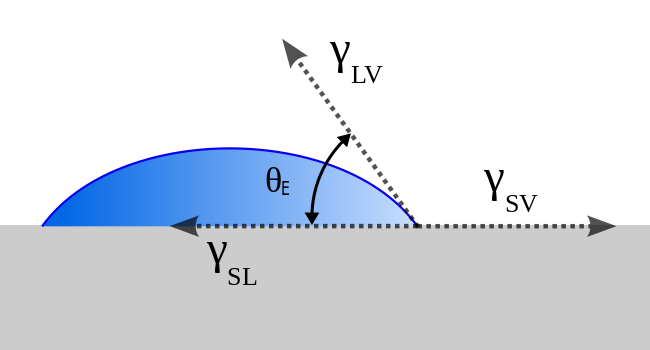
\includegraphics[scale = 0.3]{./image/Contact_angle2.png}
	\caption{Ligne triple}
	\label{fig:mesure}
\end{figure}
 A l'équilibre
Nous nous interessons en particulier au contact d'une goutte dont le support est une plaque plane. 


Le substrat est de façon général le nom donné au support sur lequel la gouttte de liquide repose (solide ou liquide).

\begin{figure}[hb]
	\centering
	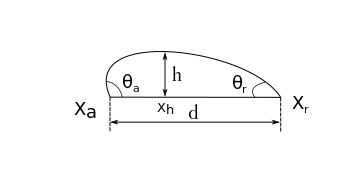
\includegraphics[scale = 0.8]{./image/rrgou.png}
	\caption{Goutte d'eau de volume $0.03$ml}
	\label{fig:mesure}
\end{figure}
Une goutte de liquide placée si 



C'est le paramètre d'étalment $S = \gamma_{SG} - \gamma_{SL} - \gamma_{LG}$ qui caractérise le mouillage lorsque la goutte est en équilibre.

En effet lorsque la goutte est en équilire nous avons en projettant les tensions de surface sur l'horizontale, on a:

\begin{equation}
	\gamma_{SG}\ = \gamma_{SL} - \gamma_{LG}\cos\theta_{E}
\end{equation}
\begin{description}
\item[$S < 0$ :] Mouillage partiel
\item[$S > 0$ :] Mouillage total
\end{description}


Lorsque la goutte est en mouvement, l'angle dynamique  est giiLa capillarité est l'étude de l'interaction en entre 2 liquides non miscinles ou entre un liqude et l'air ou en un liquide et une surface.

La tension de surface 

La capillarité étudie l'interface entre l'air et un liquide ou entre 2 liquides
non mixibles.

Le mouillage est l'action de mouiller et mouiller consiste à mettre en contact avec un liquide.

Nous nous interessons en particulier au contact d'une goutte avec un support matériel.

C'est le paramètre d'étalment $S = \gamma_{SG} - \gamma_{SL} - \gamma_{LG}$ qui caractérise le mouillage lorsque la goutte est en équilibre sur un support matériel.

\begin{description}
\item[$S < 0$ :] Mouillage partiel
\item[$S > 0$ :] Mouillage total
\end{description}

Lorsque la que est en équilire nous avons:

\[\gamma_{SG}\ = \gamma_{SL} - \gamma_{LG}\cos\theta_{E} \]

\begin{figure}[ht]
	\centering
	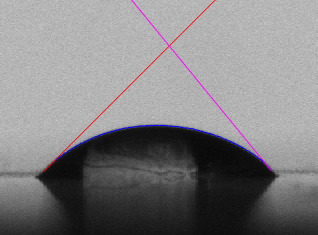
\includegraphics[scale = 0.6]{./image/crop_tvitesse=28_volume=003.png}
	\caption{Goutte d'eau de volume $0.03$ml avec $\theta_{a} = 45^{o}$ et $\theta_{r} = 50.17^{o}$}
\end{figure}

\begin{figure}[ht]
	\centering
	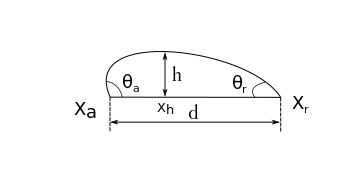
\includegraphics[scale = 0.6]{./image/rrgou.png}
	\caption{Goutte d'eau de volume $0.03$ml}
\end{figure}
\end{document}
